\chapter{Data and Preprocessing}
\label{chap:data-and-preprocessing}
\section{Datasets: NLST and DLCSD24}
The development and evaluation of computer-aided detection systems for pulmonary nodules heavily rely on comprehensive and diverse datasets. In this work, we leverage two distinct datasets: the National Lung Screening Trial (NLST) \cite{nlst_data} and the Duke Lung Cancer Screening Dataset 2024 (DLCSD24) \cite{dlcsd24}. Each dataset presents unique several slices/volumes of CT scans, annotated with pulmonary nodule locations, necessary for training and validating our detection models.

Both datasets will serve as 2D datasets, meaning that each slice of the CT scan will be treated as a separate image. The slicing will be done along the axial plane, which is the most common orientation for viewing CT scans.
The NLST dataset already comes as a collection of 2D slices on the axial plane, while the DLCSD24 dataset comes as a collection of 3D volumes that will need to be sliced along our desired plane, and possibly only a subset of slices of interest -- namely those containing nodules -- will be retained for training and evaluation.

\subsection{National Lung Screening Trial (NLST)}
The NLST is a large-scale, randomized controlled trial conducted by the National Cancer Institute (NCI) to determine if spiral computed tomography (CT) screening could reduce lung cancer mortality compared to standard chest X-ray. It enrolled over 53,000 participants at 33 sites across the United States. For the purpose of this study, the NLST dataset provides a vast collection of low-dose CT scans, which are invaluable for training nodule detection models.
Unfortunately, only a small subset of the NLST dataset includes annotations for pulmonary nodules, and these only cover malignant nodules.
After this filtering, we are left with approximately 9000 scans, each containing on average one nodule, for a total of around 9000 nodules of size greater or equal to 4 mm.
Regardless the absence of benign annotations, the NLST can be effectively utilized to teach a model to recognize nodule-like structures. Furthermore, the NLST dataset can serve as an excellent source for pre-training detection models, allowing them to learn general features of pulmonary nodules before fine-tuning on datasets with more detailed annotations.


\subsection{Duke Lung Cancer Screening Dataset 2024 (DLCSD24)}
The Duke Lung Cancer Screening Dataset (DLCS 2024) is a large-scale, annotated collection of low-dose thoracic CT scans designed to support research in lung nodule detection and cancer risk assessment using modern CT technology \cite{dlcsd24}. The dataset was compiled from screening examinations conducted at the Duke University Health System between January 2015 and June 2021, and consists of 1,613 CT volumes drawn from a pool of 2,061 patients, with additional cases reserved for future releases. Within these scans, a total of 2,487 nodules were annotated through a semi-automated pipeline in which a detection model, pre-trained on the LUNA16 dataset, generated candidate nodules that were subsequently verified and refined using radiology reports and expert review. Manual adjustments were performed by a medical student and a fellowship-trained cardiothoracic radiologist, and independent spot checks confirmed that the resulting annotations achieved an accuracy exceeding ninety percent. The dataset is released in multiple parts, with versioned updates hosted on Zenodo to ensure accessibility and reproducibility, and represents the first publicly available, large-scale screening dataset acquired with up-to-date CT protocols. As such, DLCS 2024 provides a valuable benchmark for developing and evaluating artificial intelligence models for lung nodule detection and classification in contemporary clinical practice.
Compared to the NLST, the DLCSD24 dataset offers both malignant and benign nodule annotations, despite with a severe imbalance with a ratio of approximately 1:10. The nodules in this dataset are also generally smaller, a property that makes them more challenging to detect. The DLCSD24 dataset is therefore particularly well-suited for training and evaluating nodule detection models, as it provides a more comprehensive representation of the types of nodules that may be encountered in clinical practice.

\subsubsection{Slice Extraction from 3D Volumes}
The DLCSD24 dataset is provided as a collection of 3D CT volumes. As previously stated in this chapter, we want to extract a 2D dataset from these volumes by slicing them along the axial plane. This is done by iterating through each volume, and extracting each slice as a separate image. If we were to extract all slices, we would end up with an extremely large dataset, with the majority of the data being non-informative, as most slices do not contain any nodules. To mitigate this, we use the provided annotations to identify slices that contain nodules, and only retain those slices for our 2D dataset. This results in a more manageable dataset size, while still retaining the most relevant information for nodule detection. 

\begin{figure}[h]
    \centering
    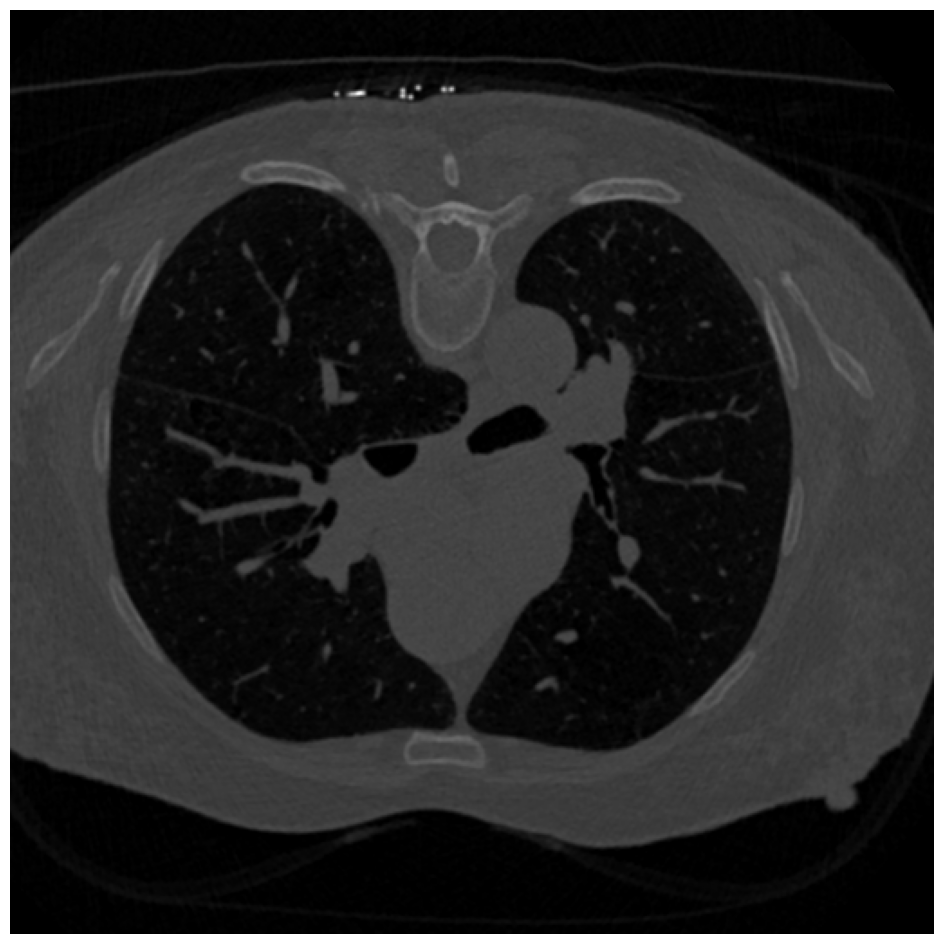
\includegraphics[width=0.6\linewidth]{images/dlcs_sample_unprocessed.png}
    \caption{Example of an unprocessed slice extracted from the DLCSD24 dataset.}
    \label{fig:dlcs-sample-unprocessed}
\end{figure}

% The size of the resulting 2D dataset depends on the thickness of the slices in the original 3D volumes, but in order to have a consistent size across all scans, we resample all volumes to have a slice thickness of 1.25mm, height and width spacing of 0.7mm, and then extract all slices containing nodules, along with a few slices before and after each nodule-containing slice to provide some context. This results in a final dataset of approximately 10,000 slices, each containing at least one nodule.

% This resampling step is crucial, as it ensures that all slices have the same resolution and spacing, which allows models to have a consistent spatial understanding of the images. 


\section{Preprocessing Pipeline}
\label{sec:preprocessing}
% Resampling, and HU clipping, explaining why we're clipping and why those ranges and not others, this is supported by the HU table.
% We might include here also discarded preprocessing steps, such as outlier removal (although it was a post-process step), and lung masking through morphological operations.

The preprocessing pipeline is a crucial step in preparing the CT scan data for effective analysis and model training. This pipeline involves several steps, including resampling, normalization, and Hounsfield Unit (HU) clipping, each of which plays an significant role in enhancing the quality and consistency of the input data and therefore quality of the detection.

\subsubsection{Resampling}
\label{sec:resampling}
CT scans can vary significantly in terms of their spatial resolution and slice thickness (a voxel might represent a differently sized parallelepiped in millimeters depending on the scan configurations), which can introduce inconsistencies when training machine learning models. To address this, we resample all CT scans to a uniform voxel (pixels for the NLST dataset) size of 1.25mm in the axial direction and 0.7mm in the coronal and sagittal directions.
These sizes were chosen according to \cite{tushar2025ailunghealthbenchmarking} as they represent a good compromise between preserving anatomical detail and managing computational resources.
This resampling is performed using bilinear interpolation, which helps to maintain the integrity of the anatomical structures while ensuring that all scans have a consistent spatial resolution.
For the DLCSD24 dataset, this resampling is performed before the slice extraction step on the entire 3D volume. Such operation is performed usign the MONAI framework \cite{monai}.

As for the NLST dataset, since it is already provided as a collection of 2D slices, we only need to ensure that each slice has the correct in-plane resolution of 0.7mm. If any slice does not meet this requirement, it is resampled using bilinear interpolation to achieve the desired resolution and it has been performed using the SimpleITK library \cite{lowekamp2013simpleitk} to extract the slices metadata and resample using its built-in resampler. The output size, given the desired spacing, original size and current spacing, is computed as follows:
$$
\text{output\_size} = \left( \left\lfloor\frac{S_1 \cdot \delta_1}{\delta_1^\prime}\right\rceil, \left\lfloor\frac{S_2 \cdot \delta_2}{\delta_2^\prime}\right\rceil, 1 \right)
$$

Where \(S_i\) is the original size along dimension \(i\), \(\delta_i\) is the original spacing along dimension \(i\), and \(\delta_i^\prime\) is the desired spacing along dimension \(i\). The output size is rounded to the nearest integer to ensure that it represents a valid number of pixels. Since the NLST dataset is already 2D, the output size for the third dimension is set to 1 as a dummy value.

\subsubsection{Hounsfield Unit Clipping}
\label{sec:hu-clipping}
Hounsfield Units (HU) are a quantitative scale for describing radiodensity in medical CT imaging. Different tissues and materials in the body have characteristic HU values, which can be used to differentiate between them. Table~\ref{tab:hu-scale} summarizes the typical HU ranges for various substances commonly found in CT scans. For our purposes, we focus on the range from -1000 HU (representing air) up to +500 HU to include soft and hard tissues, while escluding extremely high values that could correspond to implants or artifacts.
\begin{table}[h!]
    \centering
    \begin{tabular}{|l|c|}
    \hline
    \textbf{Substance} & \textbf{HU Range} \\ \hline
    Air & $-1000$ \\ \hline
    Lung & $-700 \ \text{to} \ -600$ \\ \hline
    Fat & $-120 \ \text{to} \ -50$ \\ \hline
    Water & $0$ \\ \hline
    Cerebrospinal fluid & $+15$ \\ \hline
    Renal Parenchyma & $+30$ \\ \hline
    Blood & $+13 \ \text{to} \ +75$ \\ \hline
    Muscle & $+35 \ \text{to} \ +55$ \\ \hline
    Liver & $+40 \ \text{to} \ +60$ \\ \hline
    Soft tissue, IV Contrast & $+100 \ \text{to} \ +300$ \\ \hline
    Bone (Cancellous) & $+300 \ \text{to} \ +400$ \\ \hline
    Bone (Cortical) & $+500 \ \text{to} \ +1900$ \\ \hline
    Metal & $>+3000$ \\ \hline
    \end{tabular}
    \caption{Hounsfield Unit (HU) ranges of different substances.}
    \label{tab:hu-scale}
\end{table}



